\documentclass[12pt]{extreport}

\usepackage[margin=1in]{geometry}
\usepackage{amsmath}
\usepackage{graphicx}

\title{Investigating Upwelled Water Over Spur Canyon}

\author{Rob Irwin}

\begin{document}
\maketitle

\chapter{Literature Review and Problem Definition}

\section{Description of the Juan de Fuca Eddy}

The eddy is a cyclonic feature located off the entrance to Juan de Fuca strait. It is seen in the summer as a consequence of northwesterly wind stress producing a southeastward current. This southeastward current produces upwelling conditions along the coast of Southern Vancouver Island. This upwelled water transports deeper nutrient rich water to the shelf, and plays a significant role in increasing biological productivity in this region of the northeast Pacific.

This eddy was first proposed by Tully [1942]. In Freeland and Denman [1982], the authors proposed that the eddy appears during the ``spring transition'' when prevailing alongshore winds switch from southeasterly to northwesterly and drive a southeastward current over the outer continental shelf and slop (direct quote from Foreman et al. [2008]). The upper layer of the eddy is reportedly in geostrophic (or very near geostrophic) balance -- the outward Coriolis force is balanced by the inward pressure gradient. Regionally, the Spur (or Tully) Canyon blocks mid-depth flow and disrupts this momentum balance. This blocking has the effect of reducing flow velocity, and thus Coriolis force. This causes an imbalance because the inward pressure force remains, forcing an ``up-canyon'' current to form.

In Freeland and Denman [1982], the water of the Juan de Fuca eddy was shown to be composed of California Undercurrent water. It was this deep water that was upwelled onto the shelf that formed the eddy. However, Foreman et al. [2008] suggest that ``the denser water that is upwelled to form the eddy is not solely composed of California Undercurrent water''. They suggest this because of studies of water composition in Juan de Fuca canyon showing that California Undercurrent water and coastal deep waters are present.

\section{Literature Review}

\subsection{Freeland and Denman [1982]; A topographically controlled upwelling center off southern Vancouver Island}

Observations from January 1979-June 1981 were performed to study the annual upwelling event seen off the coast of southern Vancouver Island. A motivation for this study was to determine whether oceanic regions adjacent to Vancouver Island belonged to the Alaska Gyre system, the California Current system, or neither. As stated in other studies, the summer winds in the area are ``extremely favourable for upwelling'' (citing two papers, Bakun [1975] and Nelson [1977]). The region of study is a line extending perpendicularly from Vancouver Island into the Pacific Ocean (figure 1 of article). The line does not intersect major regions of study in Foreman et al. [2008], and the line is north of the Spur Canyon rim. Stated in the introduction: La Perouse Bank is the only topographic feature with a length scale larger than the internal Rossby radius of deformation and so it is the only one likely to be able to modify substantially the large scale geostrophic flows. Current meter moorings and CTD's were used to observe the study region. The dissolved oxygen content was measured over the study period. At station 105, a significant drop in dissolved oxygen is generally observed around springtime and it is stated that ``the spring decline in oxygen is much faster than can be accounted for by biological oxygen demand.'' The dissolved oxygen levels were seen to return back to a ``normal'' state in the fall. Upwelling indices are shown. The indices are calculated as weekly averages. Not surprisingly, at station 105 (along the shelfbreak roughly), the upwelling index is periodic in nature, with positive values in the summer, and negative values in the winter.

The first clear picture of the Juan de Fuca eddy is shown in figure 5, where a contour plot of $\sigma_t$, or potential density is shown at a fixed depth. The authors state that there is a definite ``front'' in the $\sigma_t$ field -- the front appears to correspond with the depth of shelf-break in the region. A region of high $\sigma_t$ is seen to develop just north of Spur Canyon, indicating the centre of the eddy. It should be noted that the authors develop contour maps using the technique of ``objective analysis'' and cite Bretherton et al. [1976]. This is noted because the study area indicated was a perpendicular line, however the authors show area maps, well south of the line of interest.

Further in the text, the authors present a contour map of a variable, $\tau$. They describe $\tau$ as:
\begin{quote}
... a function of temperature and salinity that is orthogonal to $\sigma_t$ curves on a $T/S$ plot. Though the actual values are of no consequence it is a convenient measure of how different two water masses are that share the same $\sigma_t$ value. It is not affected by seasonal changes that might make density more or less strongly determined by salinity or temperature. If two water masses have the same $\tau$ on any given $\sigma_t$ surface, then those two water masses are identical.
\end{quote}
This is effectively what is known as \textit{spice}. 

The authors then establish that during the summer months, at station 105, the water mass at $100m$ depth is evidently California Undercurrent water. They state: 
\begin{quote}
Somehow California Undercurrent water is being raised from depth and deposited on the continental shelf. The observations that this water is low in oxygen and high in nutrients further confirm the notion that the water has been away from the surface layer for a considerable time. However, to date there have been no direct observations of the California Undercurrent this far north.
\end{quote}

It is seen to be a curious case that water so deep was raised to the surface with non-standard upwelling conditions. There are four details specified by the authors that suggest this upwelling event is not of the classical kind, but rather a special locally determined phenomena:
\begin{enumerate}
\item upwelling is considered to be a local response to local winds, however the upwelling index combined with wind observations refute this
\item depths of classical upwelling are typically only moderate depths below the shelf-break --- they cite $250m$ as the expected depth of upwelling, when in reality this event must take water from $450m$ 
\item the frequency of upwelling is expected to have the same frequency as that of the winds. Here, there is one long sustained event per year that lasts for longer than 100 days.
\item ``There should be nothing particularly special about the response at this location''. They state northern Vancouver Island sees the same wind forcing conditions, but annual cycles are much smaller magnitude than observed here.
\end{enumerate}

Current meter observations along the observation line indicate directionality and magnitude of currents at depths of $50m$ and $100m$ (figure 8 of text). Currents these depths are typically towards the northwest during downwelling, and towards the south east during upwelling. Stations CZ4 (continental slope station) and CZ3 (shelf edge station) are discussed first. In terms of directionality, the authors concisely state that the currents are ``strongly polarized parallel to the local bathymetry'', with magnitudes around $20cm/s$ in the winter. A sharp transition occurs on March 18\textsuperscript{th} 1980 at CZ3, then four days later at CZ4, in terms of current directionality. This sharp transition has been dubbed ``the spring transition''. Authors note that although one might expect the winds and currents to be in phase, the major change in wind system occured on March 8\textsuperscript{th}, considerably earlier. The following year, 1981, the wind transition occured on March 28\textsuperscript{th}, while the current transition occured around March 6\textsuperscript{th}. From the authors:
\begin{quote}
The conclusion is, therefore, that the major seasonal cycles in currents are not strongly coupled to the local wind system.
\end{quote}

For stations CZ1 and CZ2, there were some difficulties in the data, and much of the summer information was lost over the course of the study. Seasonality was still reported, however the data gives a much weaker seasonal dependence than the two more offshore stations.

Vertical shear is discussed in the following section, along with dynamic height (not summarized here).

The authors propose that because the eddy is ``always closely associated with the northern terminus of the Spur Canyon'', that the canyon is an essential component of this upwelling phenomena. They outline a sequence of events that leads to this upwelling behaviour:
\begin{enumerate}
\item in winter, shelf edge currents are northbound and the Juan de Fuca outflow current is also northbound along the coast
\item in ear spring (say mid-March) the shelf edge current reverses (the spring transition) and a cyclonic eddy is spun up on the wide continental shelf. Stratification is initially weak so vertical shear is initially small
\item the eddy is quasi-geostrophic and flows over the Spur Canyon; however, the canyon width is about half the internal Rossby radius of deformation, so the geostrophic circulation in the eddy cannot be significantly influenced by the presence of the canyon\item since in the early spring vertical shear is small, water parcels moving in the eddy experience an inward pressure gradient that is largely balanced by an outward Coriolis force. Near the bottom these forces are still felt; however, inside the Spur Canyon water parcels experience only the pressure gradient force since the horizontal motion of water parcels is suppressed by the blocking effect of the Canyon
\item the inward pressure gradient forces a weak flow up the canyon to develop which advects water from the mouth of the canyon system onto the continental shelf
\item water originally in the canyon system at the time of the spring transition flows onto the continental shelf, and accounts for the slow decline in dissolved oxygen levels seen between the spring transition and the rapid decline in oxygen levels
\item as water originating from the California Undercurrent passing the mouth of the Juan de Fuca arrives on the shelf, we observe the rapid decline in oxygen values seen in early June of each year
\item as dense water accumulates on teh shelf horizontal density gradients increase, vertical shear increases (through the thermal wind relation) and the deep inward pressure gradient decreases. If water tends to flow back down the canyon the vertical shear will decrease which will tend to restore the inward pressure gradient
\end{enumerate}

The following section attempts to prove that the classical model of wind-driven upwelling is insufficient for this specific case. It is shown that the volume of anomalous water on the shelf during summer months cannot be driven by classical upwelling. Following this proof, a toy model is created to show how deep water may be upwelled through a rectangular canyon. The depth of upwelling derived matches well with observations. However, this model neglects Coriolis forces and local effects. It is also a steady state model.

\subsection{Mackas et al. [1987]; Least Squares Multiple Tracer Analysis of Water Mass Composition}

A mathematical formulation of water mass composition is put forth (not summarized here). Instead, the results of this mass composition analysis will be shown. The important information presented in this paper is contained within table 1, and figure 3.

\begin{table}[h]
\centering
\begin{tabular}{p{.25\textwidth} p{.1\textwidth} p{.1\textwidth} p{.1\textwidth} p{.1\textwidth} p{.1\textwidth}}
\hline
& & & Source & & \\
\hline
& Juan de Fuca & Offshore & Subarctic & California Undercurrent & Coastal Deep \\
\hline
Temperature, $^\circ C$ & 9.84 & 8.75 & 4.70 & 6.90 & 5.10 \\
Salinity & 31.55 & 32.62 & 33.57 & 33.90 & 34.10 \\
Nitrate, $\mu$mol & 24.68 & 7.63 & 29.00 & 33.40 & 40.00 \\
Phosphate, $\mu$mol & 2.19 & 1.11 & 2.30 & 2.65 & 3.20 \\
Silicate, $\mu$mol & 41.76 & 12.55 & 48.00 & 52.00 & 90.00 \\
Oxygen, $mL/L^{-1}$ & 5.26 & 6.20 & 4.65 & 2.10 & 0.50 \\
\hline
\end{tabular}
\caption{Table 1 from Mackas et al. 1987}
\label{tab:mackas}
\end{table}

Five transects beginning along the coast and moving from towards the Pacific are considered in their paper. Line A transects the Washington Coast and heads directly west, offshore to the shelf break. Lines B-E begin along the coast of Vancouver Island and move south-west towards the shelf break. Line B is of primary importance to the present research, as it appears to cross a region near Spur Canyon. Each line will be analyzed for water composition based on table \ref{tab:mackas}.

It is noted in the text that the middle of lines A and B are where the upwelling focus is concentrated.

\begin{itemize}
\item \textbf{Line A} \\
Juan de Fuca water composes only a small part of the entire volume. It is confined to the top 50m and even when it is detectable, only accounts for half-or-less of the water volume.

Offshore water is more dominant away from the immediate coast, however it still composes 25-50$\%$ of the top 100m of coast water. Traces of offshore water are not apparent past 150m in depth, and most of its influence is contained in the top 100m of the water volume along this transect.

Subarctic water is not detectable along transect A.

The California Undercurrent accounts for a large portion of the water volume. In particular, the deeper water below 100m depth is $>75\%$ composed of the California Undercurrent water mass. Each measured station showed that this water mass contributed for $>50\%$ of the volume below 50m in depth. The shallower portions of the water volume show a significantly attenuated contribution from the undercurrent.

Coastal Deep water appears to be confined in a trench area along line A, however the contribution is small ($<25\%$).
\item \textbf{Line B} \\
Juan de Fuca water is a more significant contributer to the water composition of line B. The surface waters near the coast are largely sourced from the Juan de Fuca waters. Moving offshore, the contribution of JdF water decreases. There are two separated ``blobs'' of JdF water at depths of 75m and 120m, respectively, however it is unclear if this is error. Regardless, the contribution of these blobs is between $10\%$ and $25\%$.

Offshore water plays a larger role in the line B transect. As the shelf begins to break, the contribution of offshore water increases (not surprisingly). This contribution is still limited to the top 200m, even after the shelf break. On the shelf, the contribution is contained to the top 50m. There are small regions of high-contribution from offshore water, however the surface waters are not of primary interest here.

Subarctic waters are seen offshore, past the shelf break, however its contribution is small.

Once again, California Undercurrent waters dominate this line transect. In many ways, its contribution is similar to that of line A; the deeper waters are largely composed of CU water, and its contribution attenuates nearer to the surface. There are no traces of CU water for deeps shallower than 20m. The most prominant contribution 
\end{itemize}

The most relevant part of their analysis is quoted here:
\begin{quote}
Results from other time periods (not presented here) confirmed Freeland and Denman's [1982] interpretation that strong seasonal variations in the depth of isopycnal surfaces and in dissolved oxygen concentration are due to changes in the amount of upwelled Undercurrent water lying on the shelf. For example, near the middle of line B, the vertically averaged contribution from the two Undercurrent sources ranges from a winter low of about $5\%$ of the water column to a summer high of over $70\%$. The difference between these two is a minimum estimate for the fraction of shelf water that is displaced (mostly within a time span of about 50 days [see Freeland and Denman, 1982]) by deep seasonal upwelling. The actual flushing rate is certainly higher, since some of the upwelled water is itself flushed from the shelf by subsequent upwelling.
\end{quote}

The data source used for the line transects is summarized in:

\noindent Hill, S., K. Denman, D. Mackas, and H. Sefton, Ocean ecology data report: Coastal waters off southwest Vancouver Island, Spring and summer 1979, Can. Data Rep. Hydrog. Ocean Sci., 3, 118 pp., 1982a.

\noindent Hill, S., K. Denman, D. Mackas, and H. Sefton, Ocean ecology data report: Coastal waters off southwest Vancouver Island, Spring and summer 1980, Can. Data Rep. Hydrog. Ocean Sci., 4, 103 pp., 1982b.

\noindent Hill, S., K. Denman, D. Mackas, H. Sefton, and R. Forbes, Ocean ecology data report: Coastal waters off southwest Vancouver Island, Spring and summer 1981, Can. Data Rep. Hydrog. Ocean Sci., 8, 93 pp., 1983.

\subsection{Meinvielle and Johnson [2013]; Decadal water-property trends in the California Undercurrent, with implications for ocean acidification}

The article begins with a good summary of the California Current System and the origins. The CCS consists of two parts; the California Current (CC) and the California Undercurrent (CU/CUC). The CC is described as a ``shallow, narrow, meandering'' current flowing southward, fed by the North Pacific Current. The North Pacific Current is classified as: cold, fresh, nutrient-poor, oxygen-rich, and relatively high-pH. The North Pacific Current is an eastward flowing oceanic current that reaches WCVI and forms the CC. The CUC is fed by Pacific equatorial water from the south, and is described as ``warm, salty, nutrient-rich, oxygen-poor, and acidic.''

In terms of seasonal variability, the CUC is strong during the summer when upwelling occurs. Surface southward jets become enhanced by strong winds and subsurface water gets upwelled onto the shelf (although this is not the direct cause of the strong upwelling). Upwelled water originates from 100-200m in depth, near the depth of the CUC core. This core depth is defined as the $\sigma_\theta =26.6 kg\cdot m^{-3}$ surface by Lynn and Simpson [1987], but more recently as the $26.4 < \sigma_\theta < 26.5 kg \cdot m^{-3}$ surface by Gay and Cheresking [2009]. The approximate position of the CUC is estimated to be $20-25km$ offshore of the shelf break. 

Authors for this study use historical data from $1950-2012$ in the region to analyze how the CCS water composition changes over long periods. The coordinate system used is: isopycnals for the vertical coordinate, and bottom depth and latitude for horizontal coordinates. The use of bottom depth as a horizontal coordinate is justified by smoothing out multi-valued components of the coordinate; i.e. small scale features that do not follow the trend of monotonically increasing depth are not included. 

\subsection{Foreman et al. [2008]; Modeling Juan de Fuca Eddy Generation}

Authors use ROMS to investigate the formation of the reported Juan de Fuca eddy. Seven numerical experiments are considered, and are summarized in table 1 of their paper. This table is reproduced here in table \ref{tab:foreman}.

\begin{table}[h]
\centering
\begin{tabular}{| p{.05\textwidth} | p{.2\textwidth} | p{.1\textwidth} | p{.1\textwidth} | p{.1\textwidth} | p{.2\textwidth} |}
\hline 
Exp. & Initial Conditions & Winds & Tides & Estuarine Flow & Objective \\
\hline
A & summer climatology & summer upwelling & yes & yes & baseline run \\
B & summer climatology & no & no  & yes & to study the role of boundary nudging \\
C & identical profiles everywhere & summer upwelling & yes & no & to study the importance of the estuarine flow \\
D & summer climatology & summer upwelling & no  & yes & to study the importance of upwelling favourable winds \\
E & summer climatology except off the entrance of the strait & summer upwelling  & yes  & yes & to study the importance of an eddy in the initial conditions \\
F & summer climatology & no & yes & yes & to study the role of tides\\
G & summer climatology & winter & yes & yes & to study the role of winter winds \\
\hline
\end{tabular}
\caption{Table taken from Foreman et al. [2008] (table 1).}
\label{tab:foreman}
\end{table}

The experiments show that the Juan de Fuca eddy is generated with reasonable accuracy compared to several observational studies done in the area. As stated by the authors 
\begin{quote}
``... the Juan de Fuca eddy can be generated with average summer upwelling favourable winds, an average summer estuarine flow in the strait, and the four major tidal constituents. Comparisons with analyzed current meter and ADCP observations near the entrance to the strait demonstrated that the model currents are reasonably accurate, thereby giving credibility to the model dynamics and suggesting that the dynamics generating the eddy in the model are real.''
\end{quote}
However, just because the eddy is generated with these four primary considerations, the influence of each effect on the eddy was not explicitly shown. Hence, experiments B-G explore the sensitivity of the eddy to each parameter.

For simulation B, the initial conditions were taken the same, but winds and tides were turned off to investigate the role of boundary conditions in the model. The boundary conditions used were ``nudging'' conditions, where boundary values would slowly relax to climatological data. It should be noted that these boundary conditions are only applied along the northern, southern and western parts of the model domain (as the eastern boundary is determined by estuarine flow). In this simulation, a weak eddy was seen (see figure 9) in the location of the Juan de Fuca eddy, however it was much weaker than in simulation A and in observations. The authors suggested that it was only present as a result of the initial conditions. They attribute the lack of an eddy forming as a result of the lack of winds and tides. The general flow is coastally constrained and towards the northwest, as opposed to simulation A which established an offshore southeast directed flow. Because the eddy was not seen in this simulation and the strong effects of tides and winds were turned off, it was concluded that boundary nudging was not determining the existence of the Juan de Fuca eddy.

Simulation C used tides and upwelling winds but removed the influence of estuarine flow from the eastern boundary. The initial conditions used were not those used in previous simulations, but simpler --- ``identical initial temperature and salinity profiles, typical of summer conditions off the Washington coast, were specified over the entire model domain''. The absence of this eastern boundary forcing removed the strong northwest directed coastal current in simulation B. Despite this simulation establishing an eddy off the coast of Cape Flattery, it is much weaker than simulation A, and does not share the same salinity patterns as simulation A. This suggests that the eastern boundary estuarine flow condition plays a significant role in the establishment of this eddy. It is not clear why the authors used different initial conditions here, and so these results may be suspect.

Simulation D removed tidal forcing from the model, but retained upwelling winds, and reintroduced estuarine conditions into the model. The eddy developed in this simulation was much stronger than the one in simulation A, suggesting that tides had an attenuating effect on the formation of the eddy. In this simulation, the eddy moved offshore and was centered over Tully Canyon. The authors make a point to say that despite this, Tully Canyon is not the origin of this eddy, but instead the eddy is generated as a result of strong upwelling off the coast of Cape Flattery, and then moves to Tully Canyon as it grows and detaches from the coast.
Simulation E kept the forcing the same, but modified the initial conditions so that an eddy was not already present in the initialization. This was done to show that the eddy is formed as a result of forcing, not as a result of biased initial data. The eddy was shown to develop slowly, but the final output was said to be very similar to that of simulation A (in particular the salinity data and velocity fields were qualitatively identical).

Simulation F investigated the effect of the tides on the formation of the eddy. The wind forcing was turned off, but tides, estuarine flow and nudging conditions were used. It was shown that tides alone can cause enough upwelling to generate an eddy at the mouth of Juan de Fuca strait. The authors concluded that upwelling favourable winds were not a necessary component of the generation of this eddy, but played a role in intensifying the eddy.

Finally, simulation G modified the upwelling favourable winds to winter downwelling winds. A weak eddy was formed at the mouth of the strait, and so it was concluded that downwelling winds alone in the winter are not enough to suppress the formation of the Juan de Fuca eddy. 

The results of these simulations show that the Juan de Fuca eddy can be generated by: average summer upwelling favourable winds and an estuarine flow; tides and an estuarine flow; and all three mechanisms working together. It was also shown that upwelling favourable winds are not a necessity, and downwelling winds will still produce a cyclonic eddy at the mouth of the Strait of Juan de Fuca.

This study further investigates upwelling off the coast of Cape Flattery and the mechanisms that cause this upwelling. They will be summarized at a future time.

\subsection{Vindeirinho [1998]; Currents, Water Properties and Zooplankton Distribution Over a Submarine Canyon Under Upwelling-Favorable Conditions}

This summary is focusing on Chapter 2 of this thesis, title ``Juan de Fuca Canyon''. Despite the title, the study is largely focused on Spur Canyon. The primary study site is denoted as JF03 and is located near $48^\circ15' N$, $125^\circ 12' W$, essentially on top of Spur Canyon. In addition to this on-canyon site, there was also a wind measurement site at Destruction Island, $47^\circ 41' N$, $124^\circ 29' W$.

The first set of analysis focuses on the correlation of wind direction at Destruction Island to current direction at Spur Canyon. It was found that even at 30m depth, the winds and currents were only weakly correlated, and this correlation decreased with depth. In an analysis of the salinity profiles, it was found that station JF03 at 30m depth was below the surface waters and was insulated from the wind, and so this decorrelation is not unexpected.

Looking at the current moorings at 30m, 75m and 200m, it is found that the prevailing currents in the top 75m are likely inducing the deep current at 200m. The 75m mooring shows that the current there is mainly cross-canyon and south to southeastward. It is found that the current weakens in August and turns northeastward (mostly eastward). At 200m in depth, the current is almost always northward, although it is stronger in July and August. This observation supports the expected summer upwelling events. The interpretation here is that the 200m current is up-canyon as a response of the overlying 30m and 75m currents moving across-canyon.

\section{Note on Spice as a Measurement}

Spice is a commonly used quantity to describe the changing of water properties along an isopycnal surface. Water is ``spicy'' compared to a reference point if it is warmer and saltier. Water is ``mintier'' compared to a reference point if it is cooler and fresher. The mathematical definition for spice is shown in Flament [2002]. Simply speaking, it is a derived measurement chosen so that changes in spice ($\pi$) do not correlate to changes in $\sigma_\theta$. Full discussion of the state variable is available in Flament [2002].

\newpage
\section{Quick Summary of the Dynamics}

\subsubsection{Water Composition in Area Around Spur Canyon}

Studied in Mackas et al. [1987], the water around Spur and Juan de Fuca Canyons, near the shelf break is largely composed of CUC water below 50m depth (see figure 3 of Mackas et al. [1987]). Meanwhile, the surface water is composed primarily of Offshore water far away from the coast, and outflow water from Juan de Fuca Strait nearer to the coast. Subarctic and Deep Undercurrent (denoted as Coastal Deep) waters are not important in these areas. It should be noted that the data used in Mackas et al. [1987] is from August 1980, and so upwelling is expected. 

\subsubsection{California Undercurrent properties}

The California Undercurrent is a northward flowing, deep current that is not seasonally effected. It moves along the west coast of the US and Vancouver Island. Following Mackas, typical properties of the CUC are:

\begin{table}[h!]
\centering
\begin{align*}
 \hbox{Temperature:}\quad& 6.90 \hbox{ $^\circ C$}\\
 \hbox{Salinity:}\quad& 33.90 \hbox{ psu} \\
 \hbox{Nitrate:}\quad& 33.40 \hbox{ $\mu$mol} \\
 \hbox{Phosphate:}\quad& 2.65 \hbox{ $\mu$mol} \\
 \hbox{Silicate:}\quad& 52.00 \hbox{ $\mu$mol} \\
 \hbox{Oxygen:}\quad& 2.10 \hbox{ mL L$^{-1}$}
\end{align*}
\caption{Properties of the California Undercurrent, taken from Mackas, reformatted from previous table.}
\end{table}

As stated in Vindeirinho [1998], the flow in the core of the CUC is generally northwest at 0.05-0.10m/s and is situated at a depth of 200-250m. Mooring data over Spur Canyon shows that the deep current is consistent throughout the year and it is the overlying current that changes seasonally. The seasonal change in this overlying current corresponds with the spring and fall transitions in the winds, however there is typically a lag time (as demonstrated in Freeland and Denman [1982], the winds and currents transition at different times, depending on the year; ``the major seasonal cycles in currents are not strongly coupled to the local wind system''). 

Hickey [1979] documents the entire California Current System (CCS) in great detail (not summarized).

\section{Falkor Data}

\subsection{CTD Data from \textit{CTD\_GG} Directory}

There are 6 primary stations here: JFG4a, LB08, BCC0, BCC1, LC12, MB07. They are summarized in figure \ref{fig:falkor_stations}.

\begin{figure}[h]
 \centering
 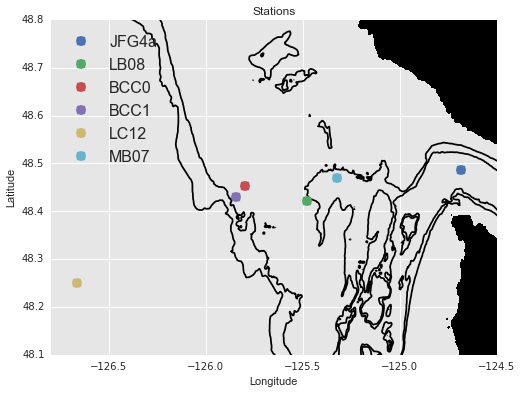
\includegraphics[width=.8\textwidth]{img/falkor_stations.png}
 \caption{Locations of Falkor stations. Contour lines are the 150m and 200m isobaths.}
 \label{fig:falkor_stations}
\end{figure}

\subsubsection{Temperature-Salinity Data}

TS diagrams were generated with corresponding 2D histogram data to see not only what the CTD data revealed about water composition, but also to see how much of each water mass was present in the data. Figure \ref{fig:falkor_histTS} shows this combined data. In addition to the raw CTD data (taken from directory \textit{CTD\_GG}), the data from Mackas et al. [1987] of the five presented water mass tracer values for temperature and salinity are overlaid. Mackas et al. [1987] report these values and use them to compare to CTD data from an August 1980 cruise.

It can be seen from this figure that California Undercurrent values from Mackas et al. [1987] (represented by the purple-ish dot) appear to correspond with the clustered parts of the histogram data (red values on the color axis). Additionally, Juan de Fuca data (blue-ish dot) only appears in the JFG4a case. All cases show that the Offshore data (green dot) appears in the data, but not to a significant amount (in the sense that the green dot always appears along the TS line, but not in regions where there is a cluster of data points). Coastal Deep water (water beneath the California Undercurrent, roughly 400m in depth) only appears in the deepest station, LC12. Subarctic water is not seen in any samples. 

\begin{figure}[h]
 \centering
 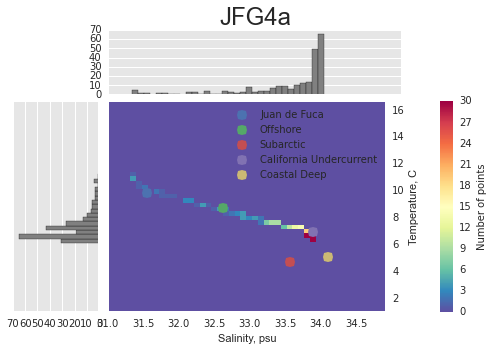
\includegraphics[width=.48\textwidth]{img/falkor_histTS_JFG4a.png}
 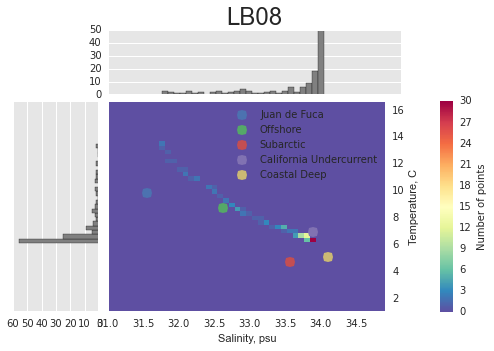
\includegraphics[width=.48\textwidth]{img/falkor_histTS_LB08.png}
 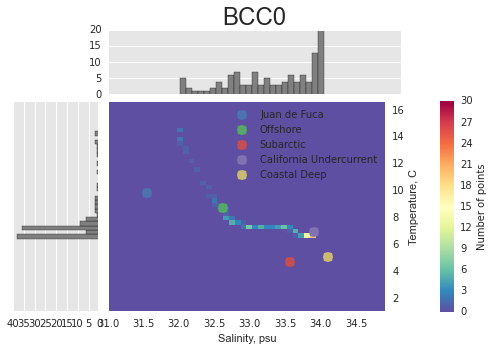
\includegraphics[width=.48\textwidth]{img/falkor_histTS_BCC0.png}
 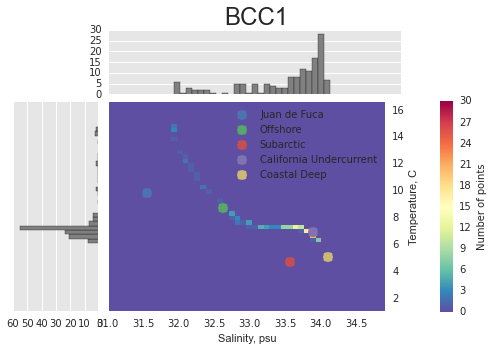
\includegraphics[width=.48\textwidth]{img/falkor_histTS_BCC1.png}
 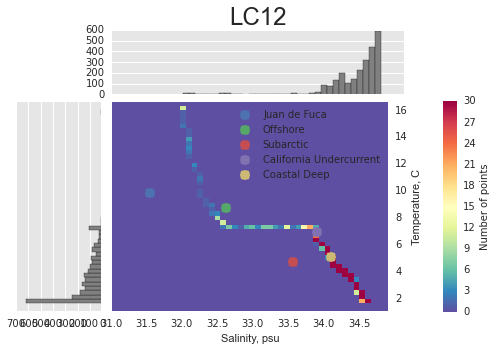
\includegraphics[width=.48\textwidth]{img/falkor_histTS_LC12.png}
 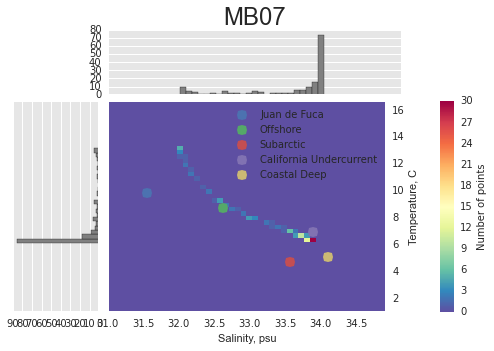
\includegraphics[width=.48\textwidth]{img/falkor_histTS_MB07.png}
 \caption{TS plots of Falkor stations. The overlaid circular markers denote the values given in Table 1 of Mackas et al. [1987]. }
 \label{fig:falkor_histTS}
\end{figure}

\subsubsection{Oxygen-Salinity Data}

Similar plots are generated by using Oxygen data from Mackas et al. [1987] and Oxygen data collected by the CTDs in the Falkor cruise. Figure \ref{fig:falkor_histOS} shows this. The oxygen values reported in Mackas et al. [1987] are significantly higher than the values collected during the Falkor cruise (with the exception of Coastal Deep water). It is noted that the Mackas et al. [1987] data was generated using historical data from 1959-1987, and so these values are certainly subject to change. However, it seems rather unlikely that these values would drop so dramatically, and so these results are to be taken with a grain of salt.

\begin{figure}[h]
 \centering
 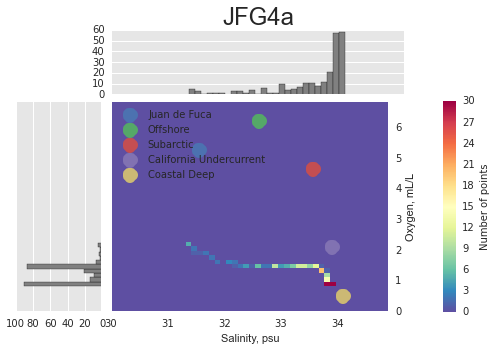
\includegraphics[width=.48\textwidth]{img/falkor_histOS_JFG4a.png}
 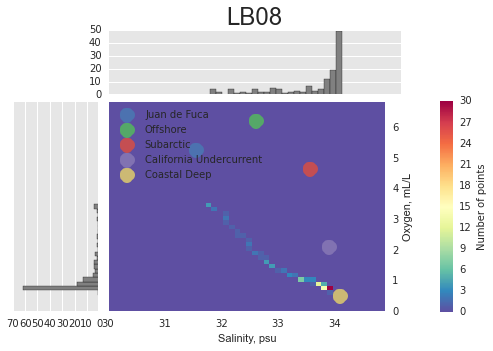
\includegraphics[width=.48\textwidth]{img/falkor_histOS_LB08.png}
 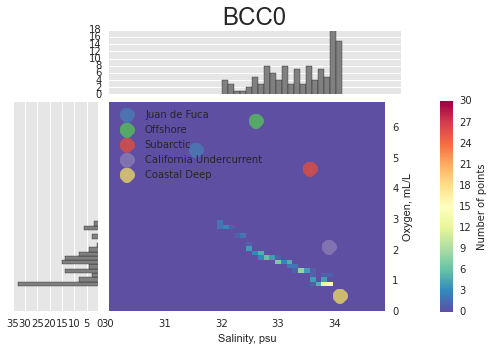
\includegraphics[width=.48\textwidth]{img/falkor_histOS_BCC0.png}
 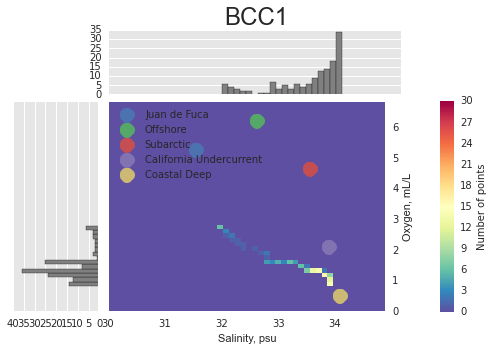
\includegraphics[width=.48\textwidth]{img/falkor_histOS_BCC1.png}
 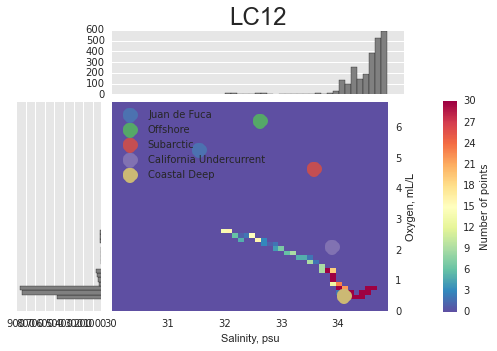
\includegraphics[width=.48\textwidth]{img/falkor_histOS_LC12.png}
 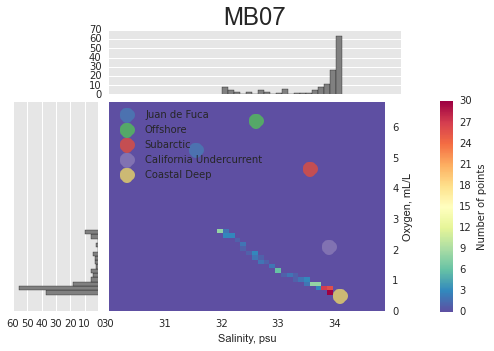
\includegraphics[width=.48\textwidth]{img/falkor_histOS_MB07.png}
 \caption{Oxygen-Salinity plots of Falkor stations. The overlaid circular markers denote the values given in Table 1 of Mackas et al. [1987]. }
 \label{fig:falkor_histOS}
\end{figure}

\end{document}
